\section{Requisitos específicos}
\label{sec:req_esp}
\subsection{Interfaces externos}

El producto consta de diferentes entradas y salida, en el caso de las entradas:\\
Destacamos un sistema de identificación de usuarios para poder ofrecer las distintas funcionalidades disponibles para cada tipo de usuario que haya en el sistema. Según sea el usuario de nuevo ingreso o ya existente en la base de datos se le solicitará unos elementos específicos.

Al nuevo usuario, independientemente de si se trata de un cliente, administrador o empleado: nombre usuario, clave personal(contraseña) y datos personales. Si el usuario ya tiene una cuenta, únicamente le hará falta hacer log in introduciendo nombre usuario y contraseña. Además, el usuario dispondrá de la capacidad de cambiar su nombre identificativo, así como su contraseña, introduciendo los datos actuales del usuario como verificación de identidad y los nuevos datos que se quieran establecer.

En el caso de ser el usuario un administrador o un empleado, podrá sancionar a un cliente introduciendo sus datos.

Destaca un menú que mostrará a los usuarios las principales funcionalidades del sistema disponibles. Las opciones variarán dependiendo de los privilegios que tenga la cuenta identificada en el sistema. En el caso de tratarse de un cliente podrá realizar la reservar, devolución o búsqueda de un producto, añadir un producto al carrito (para realizar la compra) e informar de algún desperfecto tras su compra.\\
Para todas estas funciones el usuario deberá de haber hecho log in e introducir los datos correspondientes al producto (ID). En el caso de informar de un desperfecto deberá introducir un mensaje explicando el problema. En el caso de tratarse de la compra de un producto, deberá añadir el producto al carrito e introducir su tarjeta de crédito (en el caso de que no la haya ingresado al registrarse).

Los administradores podrán añadir una nueva promoción introduciendo los datos correspondientes, así como eliminar una ya existente. Por otro lado, podrán aplicar un descuento a un producto, así como realizar actualizaciones de stock añadiendo o quitando productos. Para estas funciones será necesario que el administrador haya hecho log in e introduzca el ID del producto sobre el cual realizar los cambios.

Por otro lado, destacamos las salidas:\\
En el caso de dar de alta o baja a un usuario, cambiar el nombre o la contraseña de este, se mostrará un mensaje indicando si la operación ha tenido éxito o no y en el caso de no tenerlo, indicará el motivo.\\
Con respecto a la reserva, búsqueda de un producto, se informará si la operación ha tenido éxito y en caso de no tenerlo se indicará si el ID del producto introducido no existe o si se trata de otro problema (en el caso de realizar una compra, que la tarjeta introducida no exista o no cuente con el dinero suficiente para realizar el pago).

Búsquedas. Las búsquedas pueden ser realizadas por cualquier usuario. Las búsquedas tendrán lugar a través del modelo especifico, talla, color, etc. El resultado de las búsquedas se mostrará por pantalla con las posibles opciones según los datos introducidos.

Factura tras una compra. La compra de un producto generará un ticket el cual se mostrará en pantalla. También existe la opción de ser enviado por correo electrónico. El ticket se generará con los datos correspondientes a los productos elegidos acompañados del precio. Para ello, se debe estar registrado y haber hecho el log in.


\subsection{Requisitos funcionales}
\subsubsection{Gestión de usuarios}%USUARIOS
\begin{figure}[H]
    \centering
    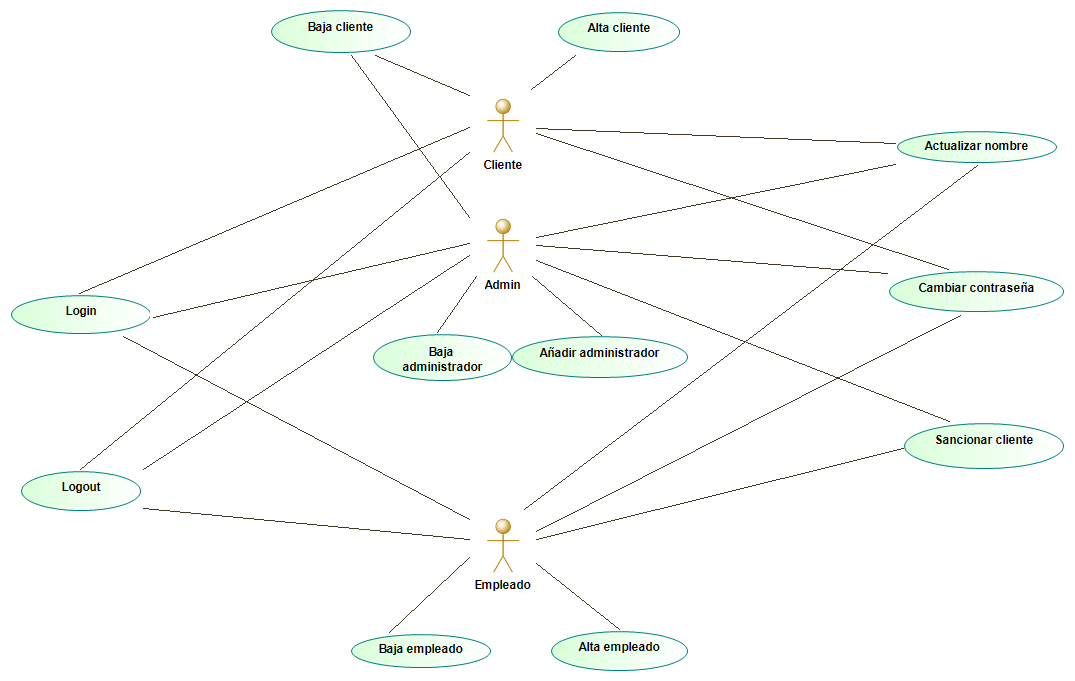
\includegraphics[width = 0.8\textwidth]{Use_Cases/Gestion_Usuarios.png}
\end{figure}
\newpage
\paragraph{Alta cliente}
\begin{table}[H]
    \centering
    \small
    \begin{tabularx}{0.8\textwidth}{|p{3.5cm}|X|}
        \hline
        \rowcolor{lightgray}
        \textbf{Nombre del caso}  & \textbf{Alta cliente}                                                                                                                       \\
        \hline
        \textbf{Descripción}      & El cliente introduce sus datos en la \gls{bd} y se da de alta.                                                                              \\
        \hline
        \textbf{Actores}          & Cliente                                                                                                                                     \\
        \hline
        \textbf{Precondición}     & Inexistente                                                                                                                                 \\
        \hline
        \textbf{Secuencia normal} & 1. El usuario selecciona la opción ``registrarse''. \newline
        2. Introducir usuario y contraseña.                                                                                                                                     \\
        \hline
        \textbf{Postcondición}    & El cliente queda dado de alta (registrado) y se muestra por pantalla el mensaje ``Usuario añadido''.                                        \\
        \hline
        \textbf{Excepciones}      & Si el usuario que se introduce ya existe en la \gls{bd} aparece por pantalla el mensaje ``Usuario ya existente, por favor introduzca otro'' \\
        \hline
    \end{tabularx}
\end{table}
\begin{figure}[H]
    \centering
    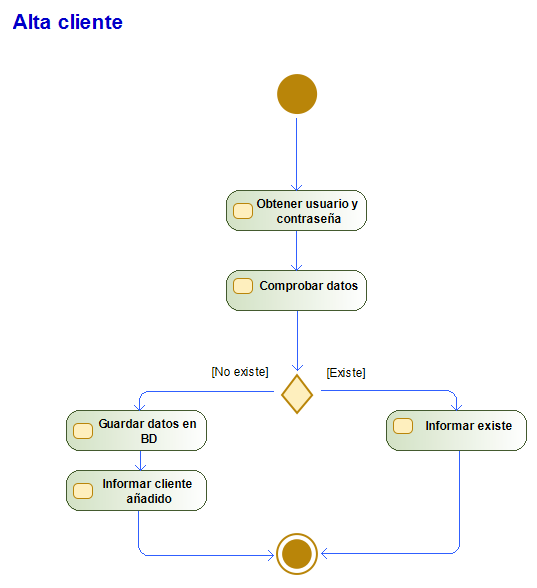
\includegraphics[width=0.8\textwidth]{Use_Cases/alta_cliente.png}
\end{figure}
\newpage
\paragraph{Baja cliente}
\begin{table}[H]
    \centering
    \small
    \begin{tabularx}{0.8\textwidth}{|p{3.5cm}|X|}
        \hline
        \rowcolor{lightgray}
        \textbf{Nombre del caso}  & \textbf{Baja cliente}                                                                                                                                \\
        \hline
        \textbf{Descripción}      & El cliente introduce sus datos en la \gls{bd} y se da de baja.                                                                                       \\
        \hline
        \textbf{Actores}          & Cliente                                                                                                                                              \\
        \hline
        \textbf{Precondición}     & El cliente debe estar dado de alta y debe existir                                                                                                    \\
        \hline
        \textbf{Secuencia normal} & 1. El cliente introduce sus datos y se loguea. \newline
        2. El cliente selecciona la opción ``Darse de baja''                                                                                                                             \\
        \hline
        \textbf{Postcondición}    & El usuario se eliminará de la \gls{bd} y aparecerá en pantalla el mensaje ``El usuario ha sido borrado correctamente''.                              \\
        \hline
        \textbf{Excepciones}      & En el caso de que los datos introducidos en la \gls{bd} no coincidan con los existentes se mostrará por pantalla el mensaje ``Usuario inexistente''. \\
        \hline
    \end{tabularx}
\end{table}
\begin{figure}[H]
    \centering
    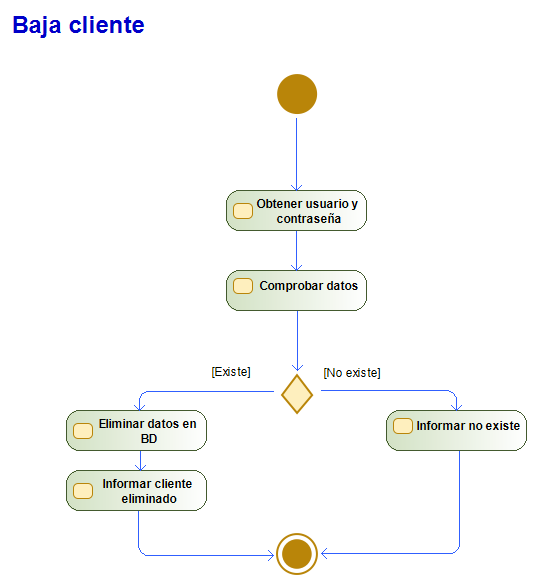
\includegraphics[width=0.8\textwidth]{Use_Cases/baja_cliente.png}
\end{figure}
\newpage
\paragraph{Añadir Administrador}
\begin{table}[H]
    \centering
    \small
    \begin{tabularx}{0.8\textwidth}{|p{3.5cm}|X|}
        \hline
        \rowcolor{lightgray}
        \textbf{Nombre del caso}  & \textbf{Alta administrador}                                                                                                                                                                                                                                                                                                                         \\
        \hline
        \textbf{Descripción}      & El usuario introduce sus datos y, si no existen ya, se guardarán en la \gls{bd} y se le darán permisos de administrador.                                                                                                                                                                                                                            \\
        \hline
        \textbf{Actores}          & Administrador                                                                                                                                                                                                                                                                                                                                       \\
        \hline
        \textbf{Precondición}     & Los datos del usuario deben ser correctos y se le tiene que haber concedido la opción de convertirse en administrador.                                                                                                                                                                                                                              \\
        \hline
        \textbf{Secuencia normal} & 1. El usuario introduce sus datos y se loguea \newline
        2. Selecciona la opción ``Obtener permisos de administrador''.                                                                                                                                                                                                                                                                                                                  \\
        \hline
        \textbf{Postcondición}    & El usuario consigue permisos de administrador.                                                                                                                                                                                                                                                                                                      \\
        \hline
        \textbf{Excepciones}      & Si el usuario introduce datos erróneos aparecerá un mensaje informando al usuario de ello. Si el usuario ya es administrador se mostrará por pantalla el mensaje ``Este usuario ya es administrador''. Si el usuario no tiene permiso para ser administrador se mostrará por pantalla el mensaje ``Usuario no válido para obtener estos permisos''. \\
        \hline
    \end{tabularx}
\end{table}
\begin{figure}[H]
    \centering
    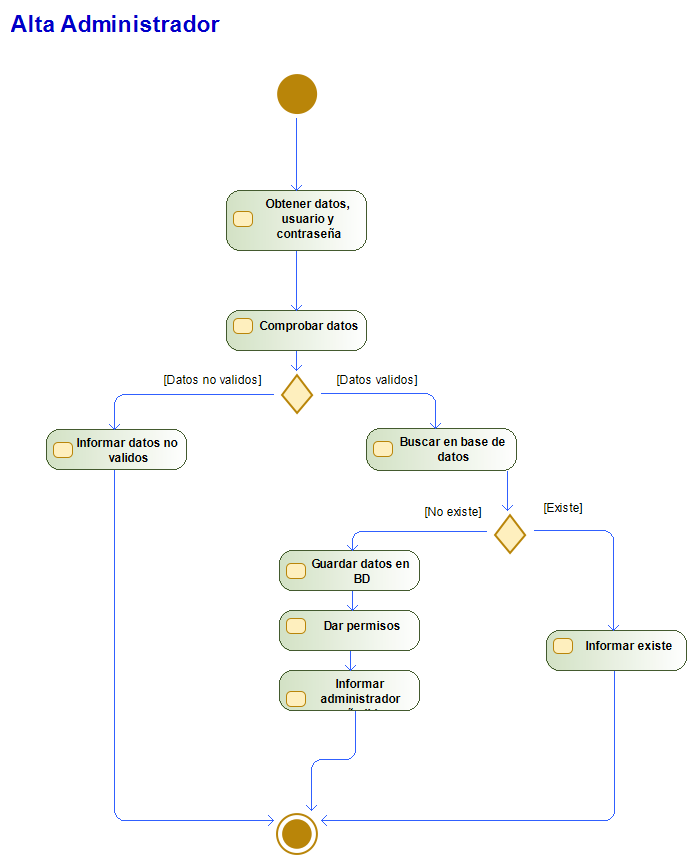
\includegraphics[width=0.65\textwidth]{Use_Cases/alta_admin.png}
\end{figure}
\newpage
\paragraph{Baja administrador}
\begin{table}[H]
    \centering
    \small
    \begin{tabularx}{0.8\textwidth}{|p{3.5cm}|X|}
        \hline
        \rowcolor{lightgray}
        \textbf{Nombre del caso}  & \textbf{Baja administrador}                                                                                            \\
        \hline
        \textbf{Descripción}      & El usuario introduce sus datos y, si existen , se le dará de baja como administrador, perdiendo sus permisos como tal. \\
        \hline
        \textbf{Actores}          & Administrador                                                                                                          \\
        \hline
        \textbf{Precondición}     & El usuario debe haberse dado de alta como administrador y existir en la \gls{bd}.                                      \\
        \hline
        \textbf{Secuencia normal} & 1. El usuario introduce sus datos y se loguea. \newline
        2. Selecciona la opción ``Darse de baja como administrador''.                                                                                      \\
        \hline
        \textbf{Postcondición}    & El usuario deja de ser administrador.                                                                                  \\
        \hline
        \textbf{Excepciones}      & Si al introducir los datos el usuario no existe se informará con el mensaje ``Usuario no encontrado''.                 \\
        \hline
    \end{tabularx}
\end{table}
\begin{figure}[H]
    \centering
    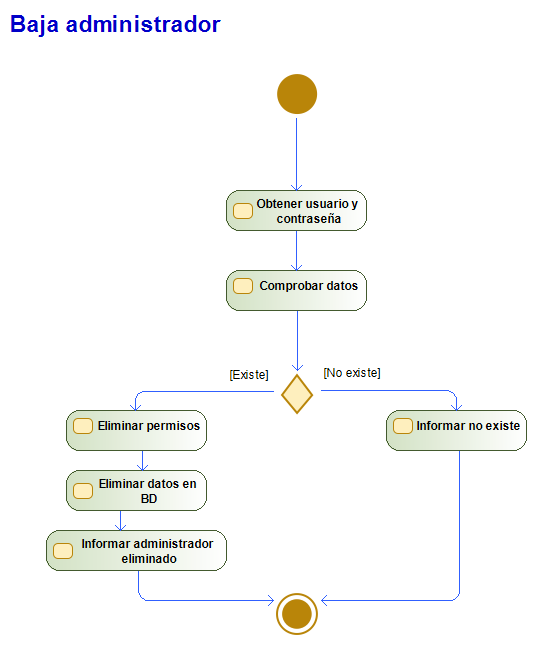
\includegraphics[width=0.8\textwidth]{Use_Cases/baja_admin.png}
\end{figure}
\newpage
\paragraph{Alta empleado}
\begin{table}[H]
    \centering
    \small
    \begin{tabularx}{0.8\textwidth}{|p{3.5cm}|X|}
        \hline
        \rowcolor{lightgray}
        \textbf{Nombre del caso}  & \textbf{Alta empleado}                                                                                         \\
        \hline
        \textbf{Descripción}      & Se introducen los datos del usuario y se registra como empleado en la \gls{bd}.                                \\
        \hline
        \textbf{Actores}          & Empleado                                                                                                       \\
        \hline
        \textbf{Precondición}     & El usuario debe tener permiso para convertirse en empleado.                                                    \\
        \hline
        \textbf{Secuencia normal} & 1. El usuario introduce sus datos y se loguea. \newline
        2. Selecciona la opción ``Darse de alta como empleado''.                                                                                   \\
        \hline
        \textbf{Postcondición}    & Los datos del empleado se han añadido en la \gls{bd} y se muestra por pantalla ``Empleado añadido con éxito''. \\
        \hline
        \textbf{Excepciones}      & Si el empleado ya existe se mostrará por pantalla el mensaje ``Este empleado ya existe''.                      \\
        \hline
    \end{tabularx}
\end{table}
\begin{figure}[H]
    \centering
    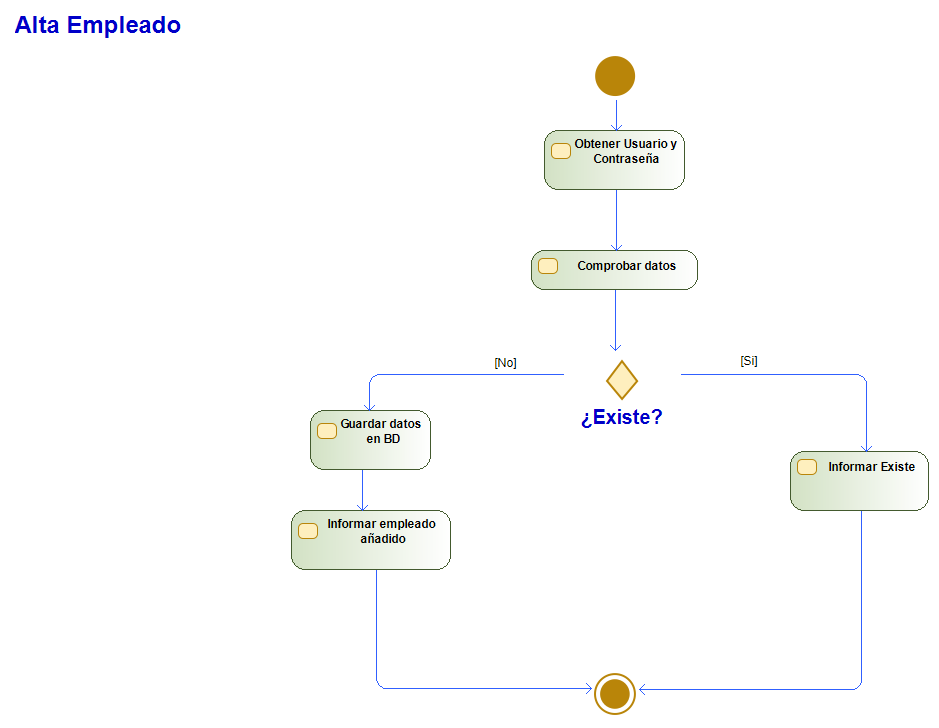
\includegraphics[width=0.8\textwidth]{Use_Cases/Alta_empleado.png}
\end{figure}
\newpage
\paragraph{Baja empleado}
\begin{table}[H]
    \centering
    \small
    \begin{tabularx}{0.8\textwidth}{|p{3.5cm}|X|}
        \hline
        \rowcolor{lightgray}
        \textbf{Nombre del caso}  & \textbf{Baja empleado}                                                                                                 \\
        \hline
        \textbf{Descripción}      & Una vez introducidos los datos, el empleado se da de baja perdiendo sus permisos como tal.                             \\
        \hline
        \textbf{Actores}          & Empleado                                                                                                               \\
        \hline
        \textbf{Precondición}     & El usuario debe haberse dado de alta como empleado.                                                                    \\
        \hline
        \textbf{Secuencia normal} & 1. Se introducen los datos del empleado en la \gls{bd}. \newline
        2. Selecciona la opción ``Dar de baja como empleado''.                                                                                             \\
        \hline
        \textbf{Postcondición}    & Los datos del empleado se borran de la \gls{bd} y se muestra por pantalla ``Empleado dado de baja con éxito''.         \\
        \hline
        \textbf{Excepciones}      & Si los datos del empleado no coinciden con los existentes se muestra por pantalla el mensaje ``Empleado inexistente''. \\
        \hline
    \end{tabularx}
\end{table}
\begin{figure}[H]
    \centering
    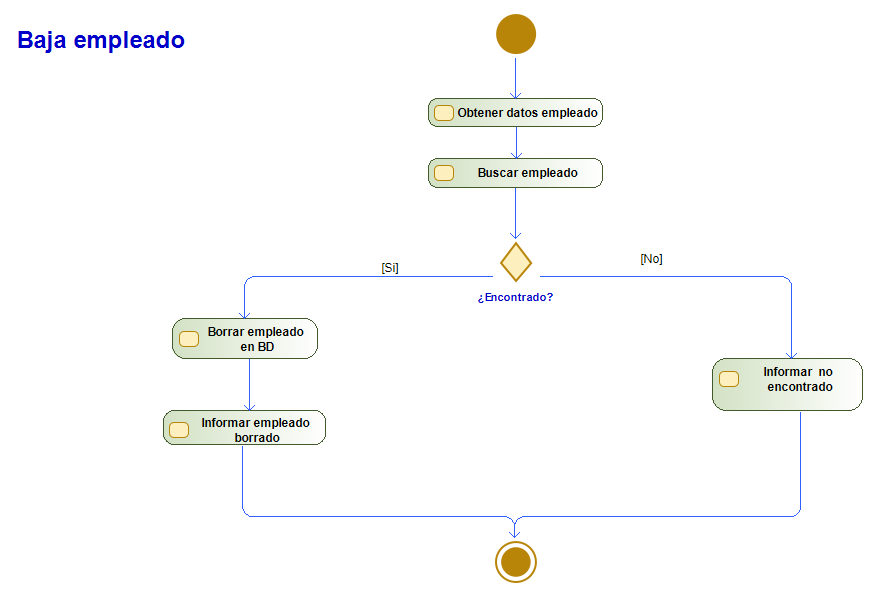
\includegraphics[width=0.8\textwidth]{Use_Cases/Baja empleado.png}
\end{figure}
\newpage
\paragraph{Sancionar cliente}
\begin{table}[H]
    \centering
    \small
    \begin{tabularx}{0.8\textwidth}{|p{3.5cm}|X|}
        \hline
        \rowcolor{lightgray}
        \textbf{Nombre del caso}  & \textbf{Sancionar cliente}                                                                                            \\
        \hline
        \textbf{Descripción}      & Se sanciona a un cliente, en caso de ser reincidente, se agrava su sanción.                                           \\
        \hline
        \textbf{Actores}          & Administrad / Empleado                                                                                                \\
        \hline
        \textbf{Precondición}     & El cliente debe existir.                                                                                              \\
        \hline
        \textbf{Secuencia normal} & 1. EL usuario (empleado o administrador) introduce sus datos y se loguea. \newline
        2. Selecciona la opción ``Sancionar cliente''.\newline
        3. Introduce los datos del cliente en cuestión y lo sanciona de manera grave o leve.                                                              \\
        \hline
        \textbf{Postcondición}    & La sanción al cliente se guarda en la \gls{bd}.                                                                       \\
        \hline
        \textbf{Excepciones}      & Si El cliente no ha cometido ninguna infracción la sanción no tendrá consecuencias y se informará de ello al usuario. \\
        \hline
    \end{tabularx}
\end{table}
\begin{figure}[H]
    \centering
    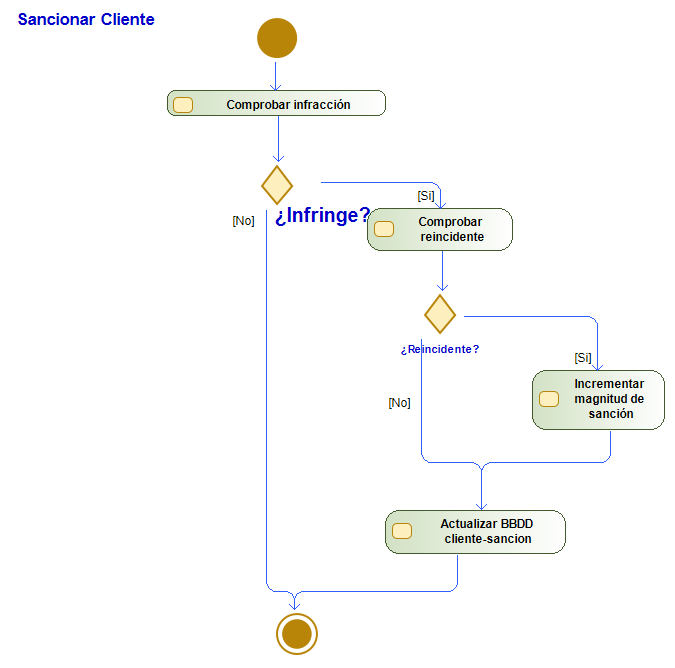
\includegraphics[width=0.8\textwidth]{Use_Cases/Sancionar Cliente.png}
\end{figure}
\newpage
\paragraph{Cambiar nombre}
\begin{table}[H]
    \centering
    \small
    \begin{tabularx}{0.8\textwidth}{|p{3.5cm}|X|}
        \hline
        \rowcolor{lightgray}
        \textbf{Nombre del caso}  & \textbf{Cambiar nombre}                                                                                                                                                    \\
        \hline
        \textbf{Descripción}      & El nombre del usuario cambia en la \gls{bd}.                                                                                                                               \\
        \hline
        \textbf{Actores}          & Administrad / Empleado / Cliente                                                                                                                                           \\
        \hline
        \textbf{Precondición}     & El usuario debe existir y dado de alta.                                                                                                                                    \\
        \hline
        \textbf{Secuencia normal} & 1. EL usuario introduce sus datos y se loguea. \newline
        2. Selecciona la opción ``Cambiar nombre''. \newline
        3. Introduce el nombre que quiera utilizar                                                                                                                                                             \\
        \hline
        \textbf{Postcondición}    & El usuario registra su nuevo nombre en la \gls{bd} y se le informa de ello.                                                                                                \\
        \hline
        \textbf{Excepciones}      & Si los datos son incorrectos se informará de ello. En el caso de que el nombre nuevo ya exista en la \gls{bd} se mostrará por pantalla el mensaje ``Nombre ya existente''. \\
        \hline
    \end{tabularx}
\end{table}
\begin{figure}[H]
    \centering
    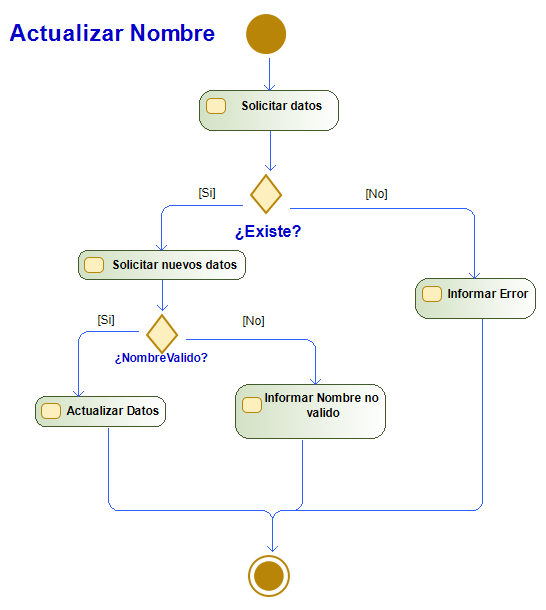
\includegraphics[width=0.8\textwidth]{Use_Cases/Actualizar Nombre.png}
\end{figure}
\newpage
\paragraph{Cambiar contraseña}
\begin{table}[H]
    \centering
    \small
    \begin{tabularx}{0.8\textwidth}{|p{3.5cm}|X|}
        \hline
        \rowcolor{lightgray}
        \textbf{Nombre del caso}  & \textbf{Cambiar contraseña}                                                                                                                                                                            \\
        \hline
        \textbf{Descripción}      & El usuario cambia la contraseña de su cuenta.                                                                                                                                                          \\
        \hline
        \textbf{Actores}          & Administrad / Empleado / Cliente                                                                                                                                                                       \\
        \hline
        \textbf{Precondición}     & El usuario debe existir y dado de alta.                                                                                                                                                                \\
        \hline
        \textbf{Secuencia normal} & 1. EL usuario introduce sus datos y se loguea. \newline
        2. Selecciona la opción ``Cambiar contraseña''. \newline
        3. Introduce la nueva contraseña                                                                                                                                                                                                   \\
        \hline
        \textbf{Postcondición}    & El usuario registra su nuevo contraseña en la \gls{bd} y se le informa de ello.                                                                                                                        \\
        \hline
        \textbf{Excepciones}      & Si los datos son incorrectos se informará de ello. En el caso de que la contraseña no cumpla con los requisitos estándar de las contraseñas se muestras por pantalla el aviso ``Contraseña inválida''. \\
        \hline
    \end{tabularx}
\end{table}
\begin{figure}[H]
    \centering
    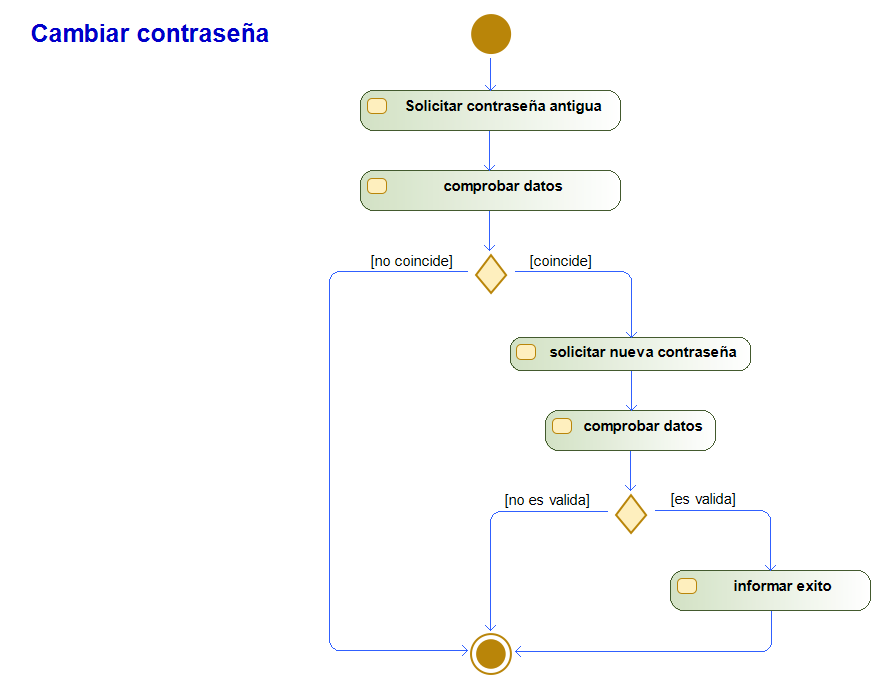
\includegraphics[width=0.8\textwidth]{Use_Cases/cambiar_contrasena.png}
\end{figure}
\newpage
\paragraph{Login}
\begin{table}[H]
    \centering
    \small
    \begin{tabularx}{0.8\textwidth}{|p{3.5cm}|X|}
        \hline
        \rowcolor{lightgray}
        \textbf{Nombre del caso}  & \textbf{Login}                                                                                                            \\
        \hline
        \textbf{Descripción}      & El usuario inicia sesión con sus datos.                                                                                   \\
        \hline
        \textbf{Actores}          & Administrad / Empleado / Cliente                                                                                          \\
        \hline
        \textbf{Precondición}     & El usuario debe existir y dado de alta.                                                                                   \\
        \hline
        \textbf{Secuencia normal} & 1. EL usuario introduce sus datos. \newline
        2. Selecciona la opción ``Iniciar sesión''. \newline                                                                                                  \\
        \hline
        \textbf{Postcondición}    & El usuario inicia sesión.                                                                                                 \\
        \hline
        \textbf{Excepciones}      & En caso de que los datos introducidos en no coincidan con los existentes en la \gls{bd}, se informará de ello al usuario. \\
        \hline
    \end{tabularx}
\end{table}
\begin{figure}[H]
    \centering
    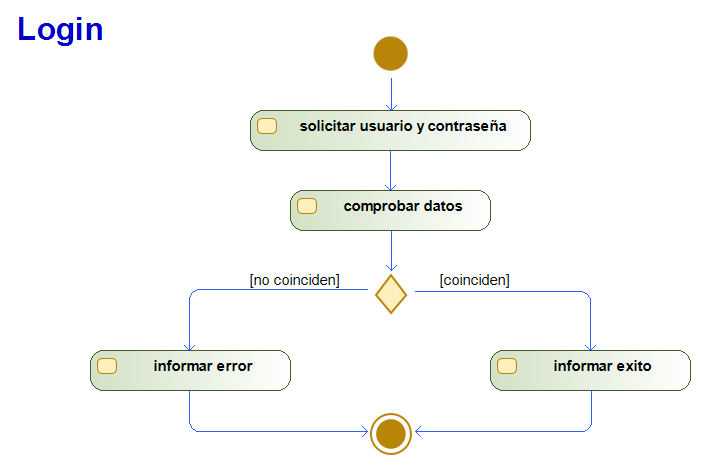
\includegraphics[width=0.8\textwidth]{Use_Cases/login.png}
\end{figure}
\newpage
\paragraph{Logout}
\begin{table}[H]
    \centering
    \small
    \begin{tabularx}{0.8\textwidth}{|p{3.5cm}|X|}
        \hline
        \rowcolor{lightgray}
        \textbf{Nombre del caso}  & \textbf{Logout}                                                                                       \\
        \hline
        \textbf{Descripción}      & El usuario cierra sesión.                                                                             \\
        \hline
        \textbf{Actores}          & Administrad / Empleado / Cliente                                                                      \\
        \hline
        \textbf{Precondición}     & El usuario debe estar logueado, existir y dado de alta.                                               \\
        \hline
        \textbf{Secuencia normal} & 1. EL usuario selecciona la opción ``Cerrar sesión''. \newline                                        \\
        \hline
        \textbf{Postcondición}    & El usuario cierra sesión.                                                                             \\
        \hline
        \textbf{Excepciones}      & La sesión de usuario se cerrará si se cierra el programa o sis e apaga el dispositivo que lo ejecuta. \\
        \hline
    \end{tabularx}
\end{table}
\begin{figure}[H]
    \centering
    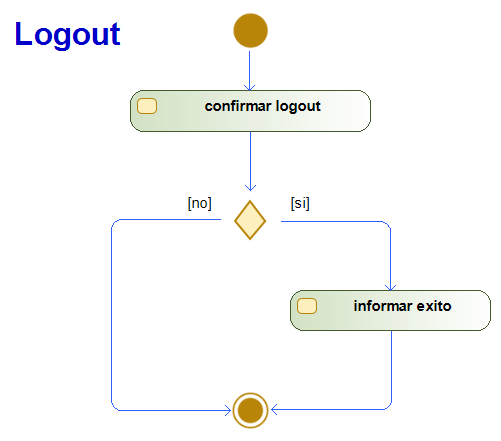
\includegraphics[width=0.7\textwidth]{Use_Cases/Logout.png}
\end{figure}
\newpage
\subsubsection{Gestión de inventario}
\begin{figure}[H]
    \centering
    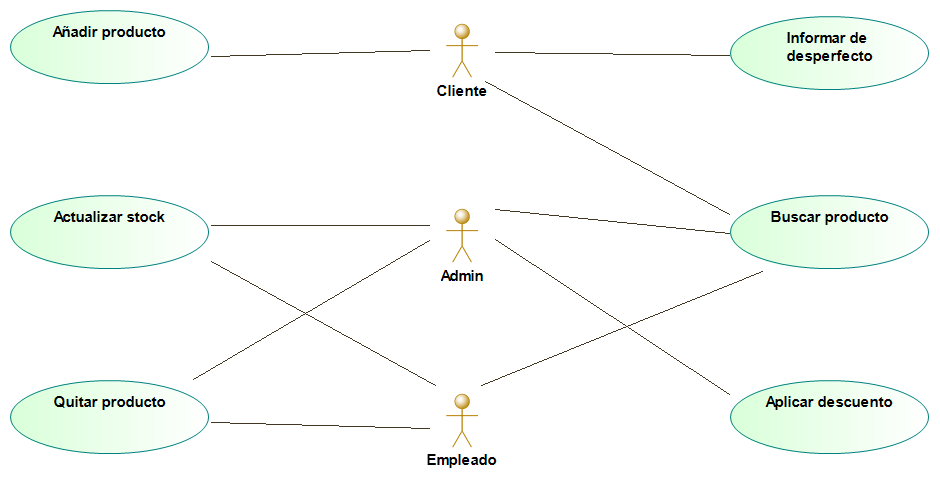
\includegraphics[width = 0.8\textwidth]{Use_Cases/gestion_de_inventario.png}
\end{figure}
\newpage
\paragraph{Añadir producto}
El usuario introduce los credenciales, incluyendo el nombre de usuario y su contraseña. Tras introducir los datos el sistema comprueba si dichos datos existen en la BD. Si existe, se comprueba el ID del producto que desea añadir, y a continuación, se comprueba los ID de los productos de su cesta si tiene alguno, de forma que si coincide con alguno, se suma una cantidad del mismo producto a la cesta, y sino, se añade un nuevo producto a la cesta.
\begin{figure}[H]
    \centering
    \includegraphics[width=0.8\textwidth]{Use_Cases/ProyectoIS_añadirProducto.png}
\end{figure}
\newpage
\paragraph{Buscar producto}
Se piden los datos del producto a buscar, si estos son correctos, se busca el producto en la BD de datos, si este existe, se muestra el producto, sino, se informa de que no existen existencias del mismo.
\begin{figure}[H]
    \centering
    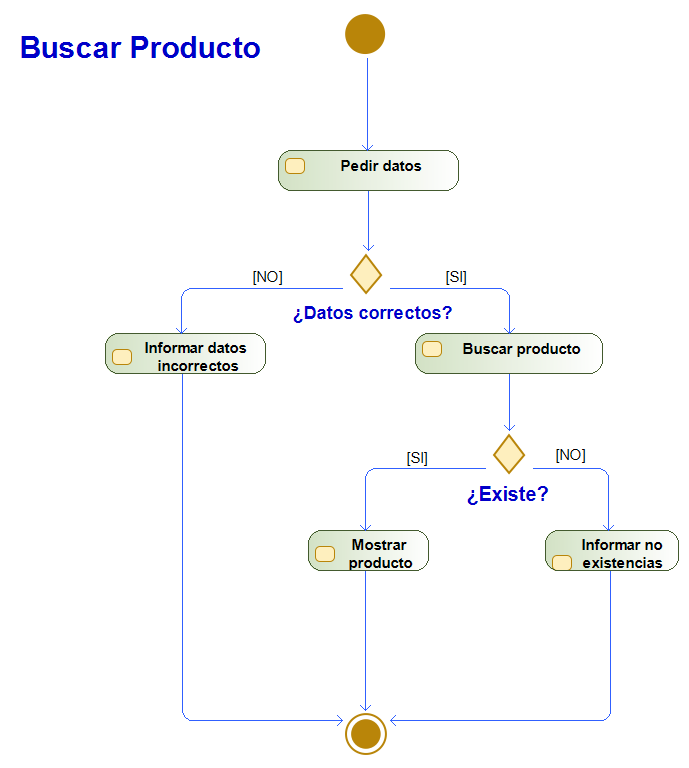
\includegraphics[width=0.8\textwidth]{Use_Cases/ProyectoIS_BuscarProducto.png}
\end{figure}
\newpage
\paragraph{Actualizar stock}
Se solicitan los datos de administrador, o empleado, si son correctos, se comprueba el ID del producto a añadir, y se solicita una modificación en la BD, si esta es aprobada, se actualiza la BD, sino se informa de que no se ha podido actualizar la BD.
\begin{figure}[H]
    \centering
    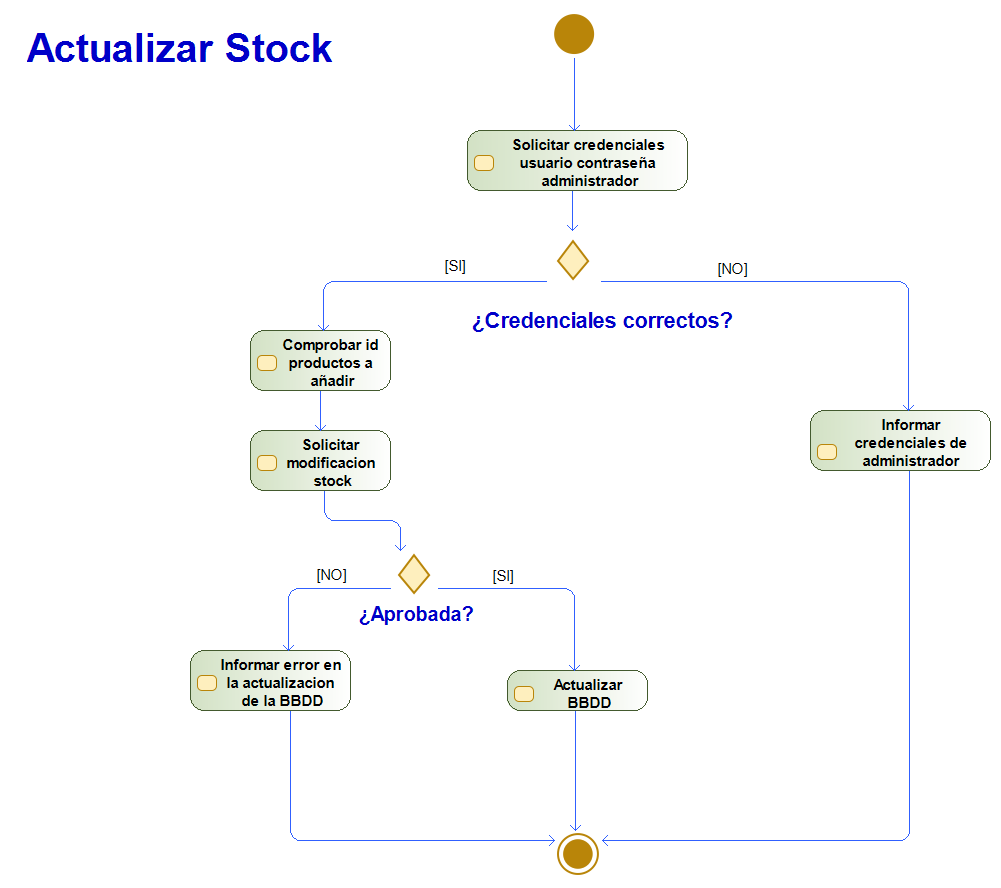
\includegraphics[width=0.8\textwidth]{Use_Cases/ProyectoIS_ActualizarStock.png}
\end{figure}
\newpage
\paragraph{Quitar producto}
Se solicita la contraseña y usuario de administrador. Si estos son correctos, se busca el producto a eliminar, y se solicita modificar la BD, si es aprobada la solicitud, se elimina dicho producto de la BD, y se informa de que se a quitado. Sino, se informa de que no se ha permitido la modificación.
\begin{figure}[H]
    \centering
    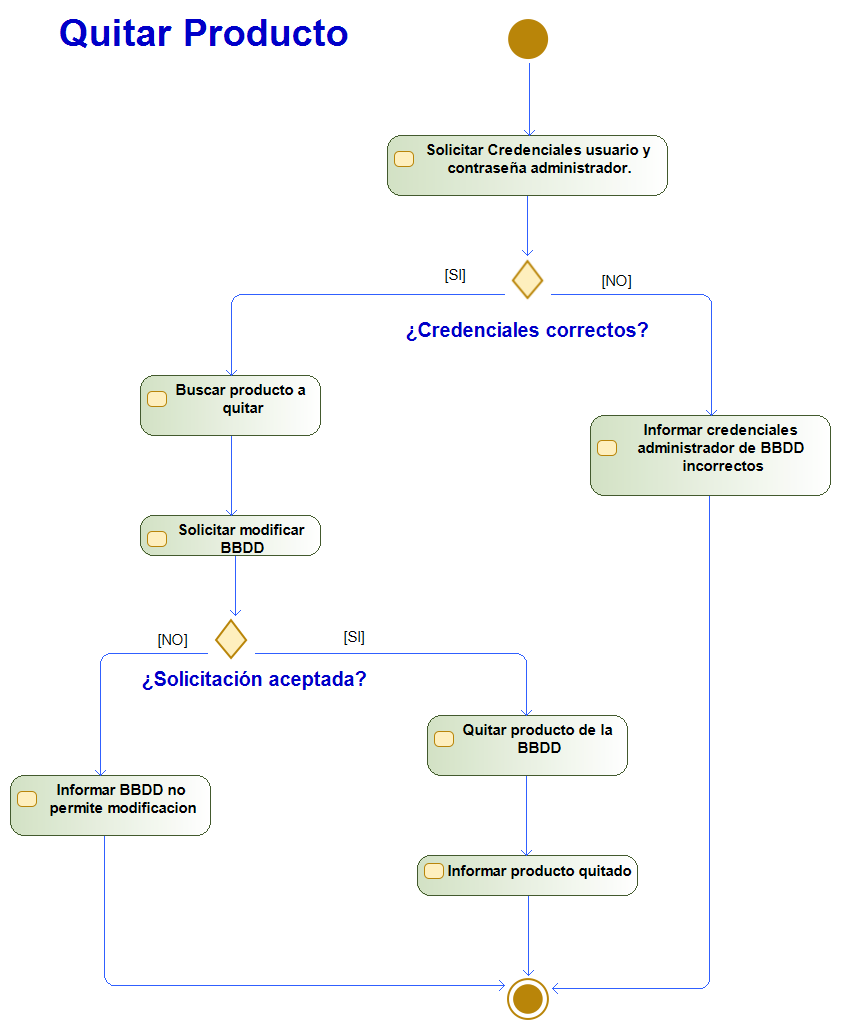
\includegraphics[width=0.8\textwidth]{Use_Cases/ProyectoIS_QuitarProducto.png}
\end{figure}
\newpage
\paragraph{Aplicar descuento}
Ingresar usuario y contraseña, comprobar si la persona está registrada en la \gls{bd}. Si el usuario no existe sale. Si el usuario existe, selecciona la opción de descuentos, verifica si el cliente tiene derecho a un descuento, si el usuario no posee ninguna opción a descuenta sale, y si tiene opción a descuento lo aplica al producto y actualiza el precio final del producto o compra total.
\begin{figure}[H]
    \centering
    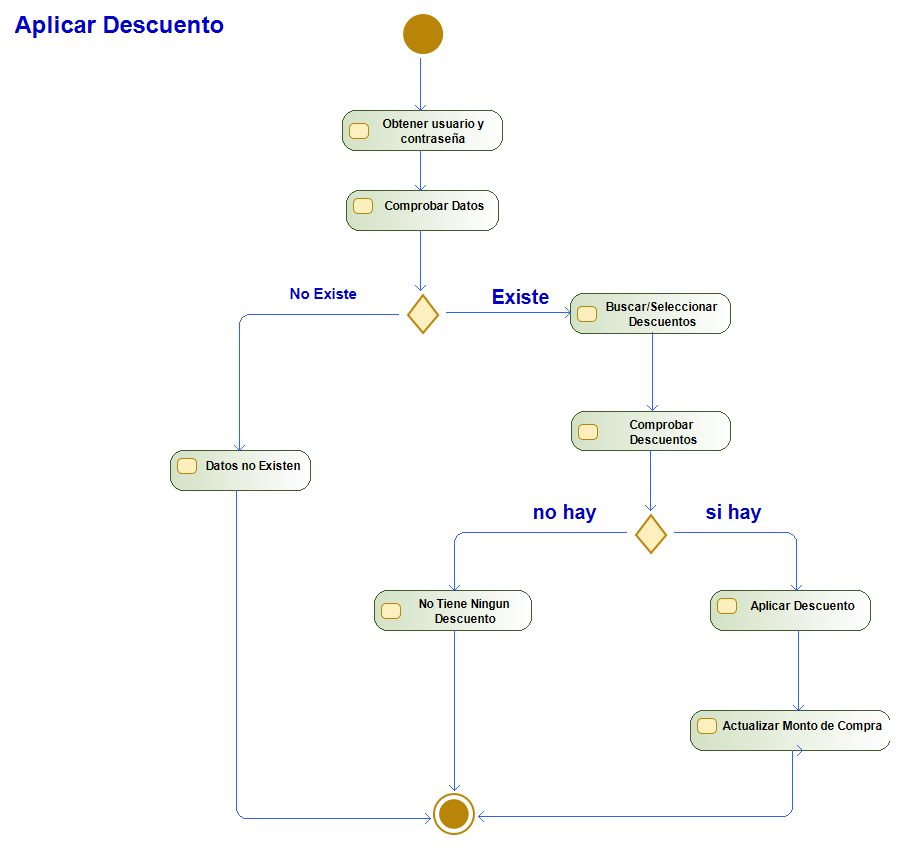
\includegraphics[width=0.8\textwidth]{Use_Cases/aplicar_descuento.png}
\end{figure}
\newpage
\paragraph{Informar de desperfecto}
Ingresar usuario y contraseña, comprobar si la persona está registrada en la \gls{bd}. Si el usuario no existe sale. Si el usuario existe, selecciona un artículo, escribe el informe acerca de los desperfectos del mismo y al final lo envía.
\begin{figure}[H]
    \centering
    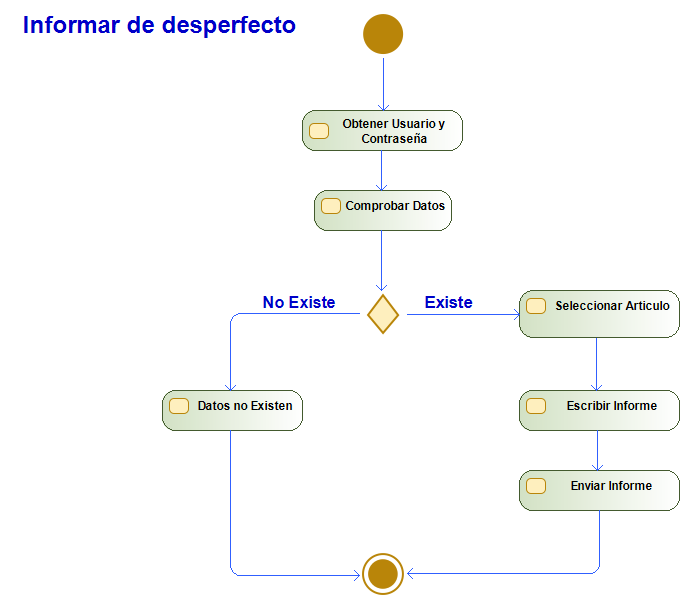
\includegraphics[width=0.8\textwidth]{Use_Cases/informar_de_desperfecto.png}
\end{figure}
\newpage
\subsubsection{Gestión de pedidos}

\begin{figure}[H]
    \centering
    \includegraphics[width=0.8\textwidth]{Use_Cases/gestion de pedidos.png}
\end{figure}
\newpage
\paragraph{Añadir promoción}
Ingresar usuario y contraseña, comprobar si la persona está registrada en la \gls{bd}. Si el usuario no existe sale. Si el usuario existe, consulta la lista de los productos en la \gls{bd}, se selecciona el producto(s) que se quiere promocionar, aplico la promoción, y actualizo el precio final del producto con la promoción incluida.
\begin{figure}[H]
    \centering
    \includegraphics[width=0.8\textwidth]{Use_Cases/añadir_promocion.png}
\end{figure}
\newpage
\paragraph{Quitar promoción}
Se obtienen los datos del administrador y se comprueba si existe. Si existe, podrá consultar dicha promoción y eliminarla, al terminar se informará del éxito de la operación. Por el contrario si no se encuentra el usuario, se informará de que se ha producido un error.
\begin{figure}[H]
    \centering
    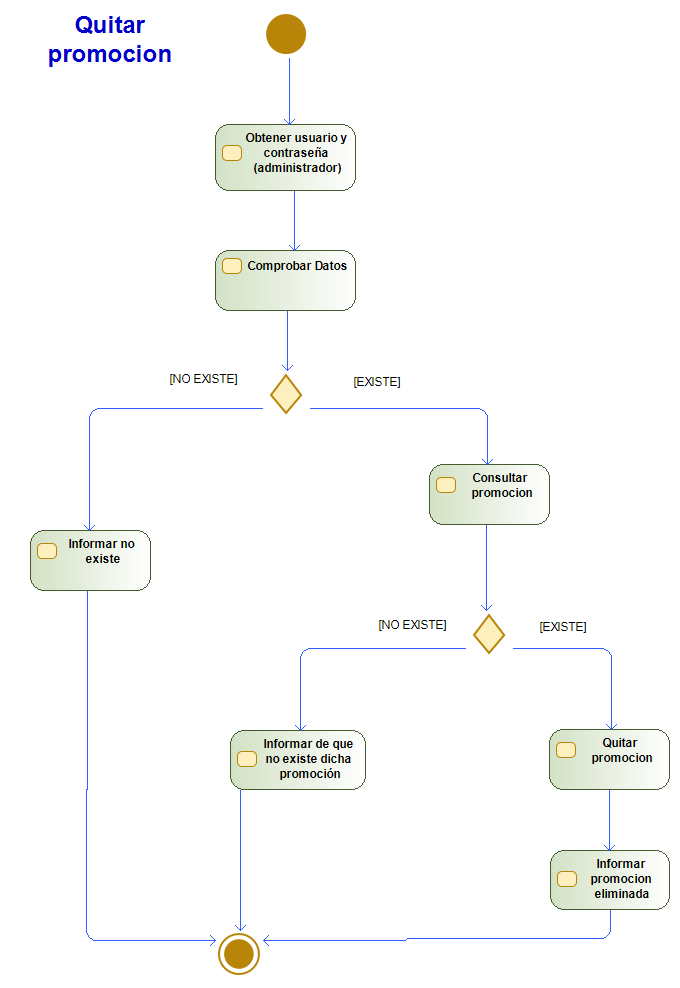
\includegraphics[width=0.8\textwidth]{Use_Cases/quitar_promocion.png}
\end{figure}
\newpage
\paragraph{Compras}
Se introduce el nombre de usuario y la contraseña del cliente. Tras introducir los datos el sistema determina si son correctos o no. Si son correctos el usuario podrá añadir productos a su cesta y cuando quiera comprar alguno, se comprobará si tiene suficiente dinero en el monedero virtual, si lo tiene, se informará del éxito de su compra si no, se informará de saldo insuficiente. En el caso de no existir el usuario, se informará de ello.
\begin{figure}[H]
    \centering
    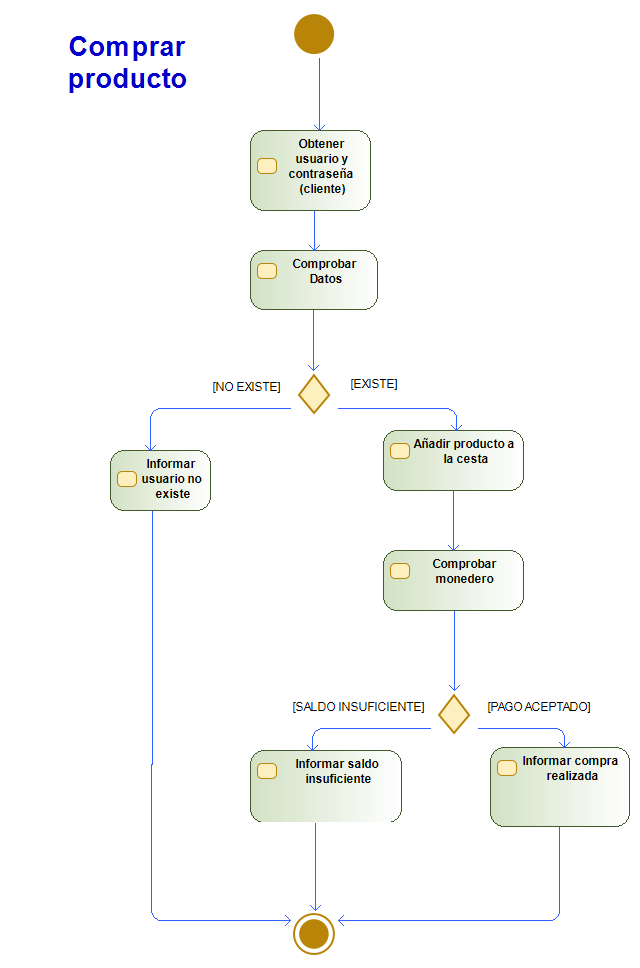
\includegraphics[width=0.8\textwidth]{Use_Cases/comprar_producto.png}
\end{figure}
\newpage
\paragraph{Devolución de pedido}
Se introduce el usuario y la contraseña del cliente. Si existe, podrá consultar sus productos comprados y proceder a su devolución, en tal caso, el saldo de dicho producto comprado volverá al monedero virtual de dicho cliente. En caso de no existir dicho usuario, se informará de ello.
\begin{figure}[H]
    \centering
    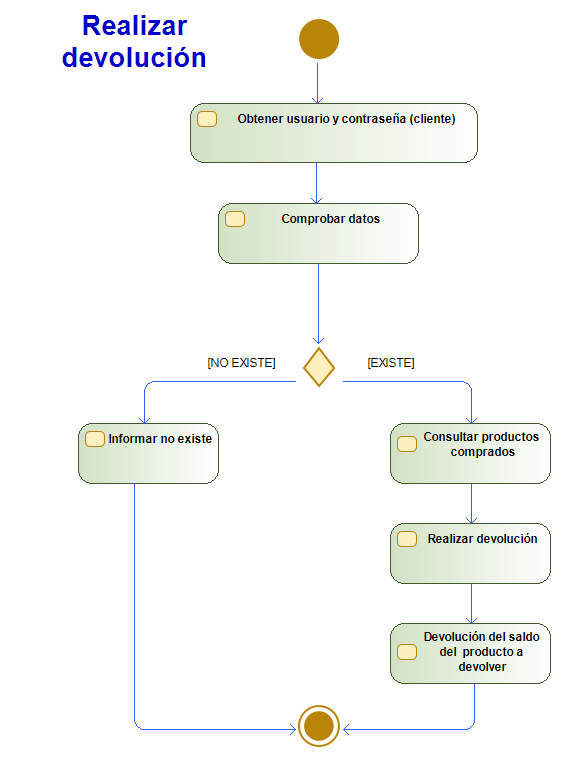
\includegraphics[width=0.8\textwidth]{Use_Cases/realizar_devolucion.png}
\end{figure}
\newpage
\paragraph{Reservar producto}
Se obtiene el usuario y contraseña del usuario y se comprueban en la \gls{bd}. Si se encuentran, el cliente podrá consultar y reservar dicho producto en el caso de que tenga suficiente saldo en su monedero virtual, en tal caso se informará del éxito del producto reservado, si no, se informará al cliente de saldo insuficiente. En el caso de no existir usuario se informará de ello.
\begin{figure}[H]
    \centering
    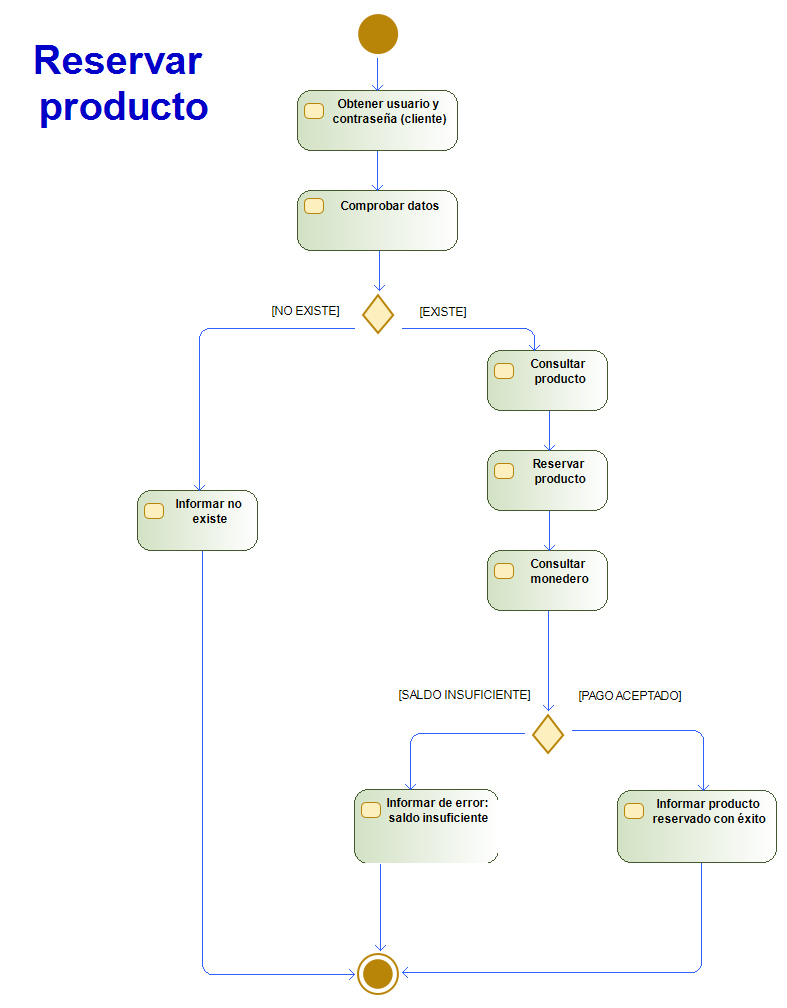
\includegraphics[width=0.8\textwidth]{Use_Cases/reservar_producto.png}
\end{figure}
\newpage
\subsection{Requisitos de rendimiento}
Las operaciones de modificación de datos serán accesibles desde un mismo sitio físico, aunque en distintas máquinas, por ello la base de datos solo debe ser modificable desde un \gls{host} local. Los datos serán accesibles para lectura desde internet.
\subsection{Requisitos sobre la persistencia de datos}
\label{sec:req_pers_dat}
\noindent\begin{tabularx}{\textwidth}{ l X }
    % \hline
    Producto-Cliente               & ``Un cliente no podrá comprar productos mientras esté sancionado"                                                \\
    Empleado-Producto              & ``El Empleado podrá dar de alta productos"                                                                       \\
    Empleado-Producto              & ``El Empleado podrá dar de baja productos"                                                                       \\
    Empleado-Producto              & ``El Empleado podrá modificar los datos de los juegos"                                                           \\
    Administrador-Producto-Cliente & ``El administrador podrá sancionar al cliente en caso de devolución fraudulenta del producto"                    \\
    Administrador-Empleado-Cliente & ``El administrador podrá cambiar las credenciales de los clientes y empleados bajo la demanda de dicho usuario'' \\
\end{tabularx}
\subsection{Restricciones de diseño}
El servidor sólo estaría disponible para ordenadores con Windows y Linux dado que este no cuenta con soporte para dispositivos Android ni dispositivos de la marca Apple.
\subsection{Atributos del sistema software}
La funcionalidad del programa estará acorde a los casos de uso en todo momento.
\begin{itemize}
    \item\textbf{Fiabilidad:} el programa asegurará que los pedidos se hagan de manera correcta. En caso de haber algún problema se podrá contactar con empleados y administradores.
    \item\textbf{Disponibilidad:} los usuarios podrán acceder en todo momento a las funcionalidades del sistema ya que la base de datos estará en un servidor dedicado. Solo se hará inaccesible cuando haya mantenimiento o actualizaciones del sistema.
    \item\textbf{Seguridad:} los datos de clientes, empleados y administradores estarán encriptados para poder asegurarlos frente a ataques externos. Toda la transferencia de datos se hará por protocolo \gls{https} para evitar fugas de datos.
    \item\textbf{Mantenibilidad:} durante el desarrollo del sistema se hará una buena documentación para que el personal que entre al proyecto pueda entender el código y su funcionalidad sin demasiada dificultad. También se hará uso de sistemas de control de versiones como git para poder revertir versiones si fuese necesario.
\end{itemize}
